%%%%%%%%%%%%%%%%%%%%%%%%%%%%%%%%%%%%%%%%%%%%%%%%%%%%%%%%%%%%%%%%%%%%%%%%%%%%
% AGUtmpl.tex: this template file is for articles formatted with LaTeX2e,
% Modified November 2013
%
% This template includes commands and instructions
% given in the order necessary to produce a final output that will
% satisfy AGU requirements.
%
% PLEASE DO NOT USE YOUR OWN MACROS
% DO NOT USE \newcommand, \renewcommand, or \def.
%
% FOR FIGURES, DO NOT USE \psfrag
%
%%%%%%%%%%%%%%%%%%%%%%%%%%%%%%%%%%%%%%%%%%%%%%%%%%%%%%%%%%%%%%%%%%%%%%%%%%%%
%
% All questions should be e-mailed to latex@agu.org.
%
%%%%%%%%%%%%%%%%%%%%%%%%%%%%%%%%%%%%%%%%%%%%%%%%%%%%%%%%%%%%%%%%%%%%%%%%%%%%
%
% Step 1: Set the \documentclass
%
% There are two options for article format: two column (default)
% and draft.
%
% PLEASE USE THE DRAFT OPTION TO SUBMIT YOUR PAPERS.
% The draft option produces double spaced output.
%
% Choose the journal abbreviation for the journal you are
% submitting to:

% jgrga JOURNAL OF GEOPHYSICAL RESEARCH
% gbc   GLOBAL BIOCHEMICAL CYCLES
% grl   GEOPHYSICAL RESEARCH LETTERS
% pal   PALEOCEANOGRAPHY
% ras   RADIO SCIENCE
% rog   REVIEWS OF GEOPHYSICS
% tec   TECTONICS
% wrr   WATER RESOURCES RESEARCH
% gc    GEOCHEMISTRY, GEOPHYSICS, GEOSYSTEMS
% sw    SPACE WEATHER
% ms    JAMES
% ef    EARTH'S FUTURE
%
%
%
% (If you are submitting to a journal other than jgrga,
% substitute the initials of the journal for "jgrga" below.)

\documentclass[draft,ms]{agutexSI}

\usepackage{rotating}


% Author names in capital letters:
\authorrunninghead{HUANG ET AL.}

% Shorter version of title entered in capital letters:
\titlerunninghead{IRRIGATION IMPACTS IN VR-CESM}

%Corresponding author mailing address and e-mail address:
%\authoraddr{Corresponding author: A. B. Smith,
%Department of Hydrology and Water Resources, University of
%Arizona, Harshbarger Building 11, Tucson, AZ 85721, USA.
%(a.b.smith@hwr.arizona.edu)}

\begin{document}

%% ------------------------------------------------------------------------ %%
%
%  TITLE
%
%% ------------------------------------------------------------------------ %%

%\includegraphics{agu_pubart-white_reduced.eps}


\title{Supporting Information for ``Irrigation impacts on California's climate with the variable-resolution CESM''}

%% ------------------------------------------------------------------------ %%
%
%  BEGIN ARTICLE
%
%% ------------------------------------------------------------------------ %%

% The body of the article must start with a \begin{article} command
%
% \end{article} must follow the references section, before the figures
%  and tables.

\begin{article}

%% ------------------------------------------------------------------------ %%
%
%  TEXT
%
%% ------------------------------------------------------------------------ %%



\noindent\textbf{Contents of this file}
%%%Remove or add items as needed%%%
\begin{enumerate}
\item Figure S1
\item Figure S2
\item Figure S3
%if Tables are larger than 1 page, upload as separate excel file
\end{enumerate}
\ \\

\noindent\textbf{Introduction}


This supplement to the manuscript includes:

\begin{itemize}

\item[(Figure S1)] The irrigated water of IRG run, and the precipitation for both NRG and IRG runs over each of the four seasons, averaged over the period 1980-2005. 

\item[(Figure S2)] The geopotential height at 500 hPa for all the simulations averaged over JJA from 1980-2005.

\item[(Figure S3)] The averaged JJA Precipitation, low-level cloud, near-surface specific humidity and convective available potential energy (CAPE) of all the simulations and their differences with t-test results for year 1980-2005 period.

\end{itemize}


%%% End of body of article:
%%%%%%%%%%%%%%%%%%%%%%%%%%%%%%%%%%%%%%%%%%%%%%%%%%%%%%%%%%%%%%%%
%
% Optional Notation section goes here
%
% Notation -- End each entry with a period.
% \begin{notation}
% Term & definition.\\
% Second term & second definition.\\
% \end{notation}
%%%%%%%%%%%%%%%%%%%%%%%%%%%%%%%%%%%%%%%%%%%%%%%%%%%%%%%%%%%%%%%%


%% ------------------------------------------------------------------------ %%
%%  REFERENCE LIST AND TEXT CITATIONS
%
% Either type in your references using

%% ------------------------------------------------------------------------ %%
%
%  END ARTICLE
%
%% ------------------------------------------------------------------------ %%
\end{article}
\clearpage

 
\begin{figure}
\setfigurenum{S1}
\begin{center}
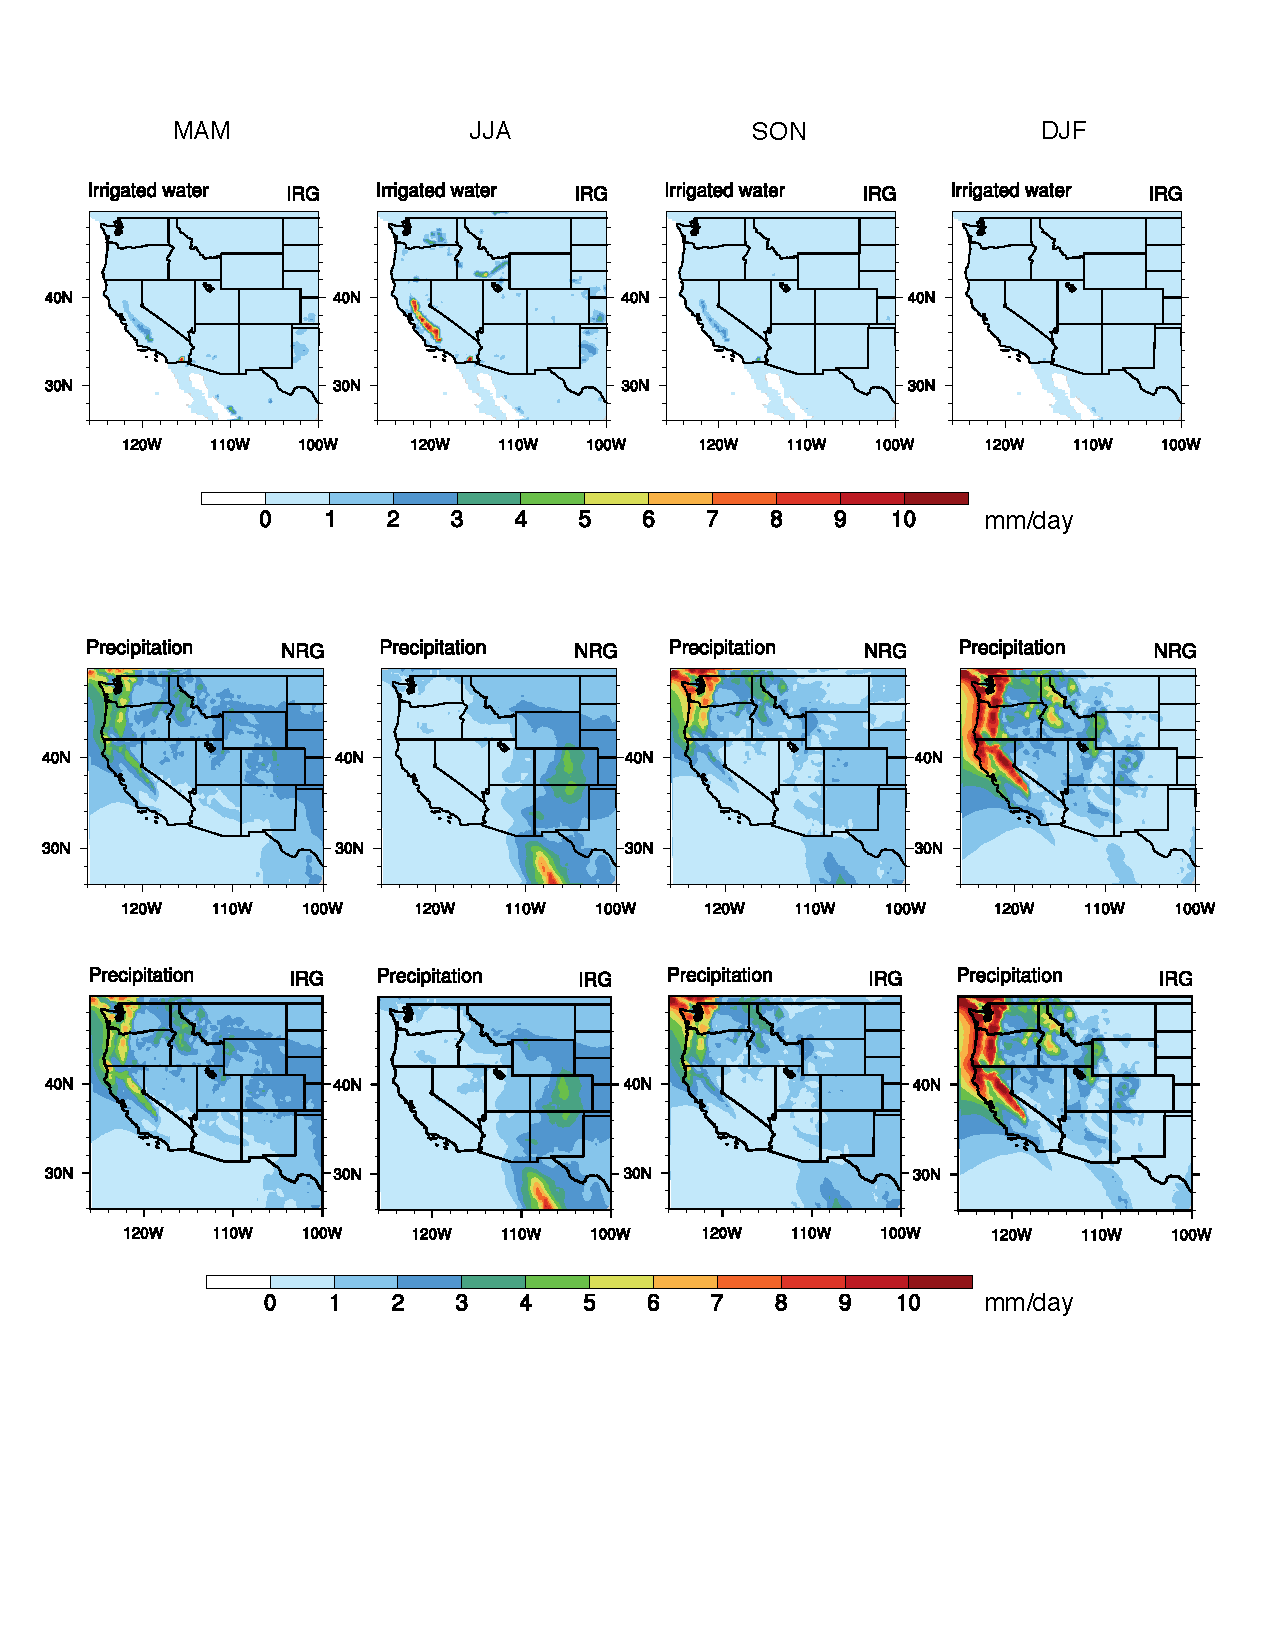
\includegraphics[width=6in]{irrigated_water_and_precipitation_4seasons.pdf}
\caption{Irrigated water from IRG, and precipitation for both NRG and IRG for each of the four seasons, as averaged over the period 1980-2005.}
\end{center}
\end{figure}

\begin{figure}
\setfigurenum{S2}
\begin{center}
\includegraphics[width=6in]{geopotential_height_500hPa_JJA.pdf}
\caption{Geopotential height at 500 hPa for all simulations (averaged over JJA from 1980-2005).}
\end{center}
\end{figure}

\begin{figure}
\setfigurenum{S3}
\begin{center}
\includegraphics[width=6in]{irrig_discussion_vs_Lo2013.pdf}
\caption{Precipitation, low-level cloud, near-surface specific humidity and CAPE for all simulations and their differences with t-test results (averaged over JJA from 1980-2005).}
\end{center}
\end{figure}

\end{document}

